\documentclass[final,3p,times,onecolumn]{elsarticle}

\usepackage{amssymb}
\usepackage{lineno}
\usepackage{amsthm}
\usepackage{amsmath}
\usepackage{algorithmic}
\usepackage{algorithm}
\usepackage{graphicx}
\usepackage{textcomp}
\usepackage{xcolor}
\usepackage{subcaption}
\usepackage{amsfonts}
\usepackage{booktabs}

\journal{MPhil in Scientific Computing}

\begin{document}

\begin{frontmatter}

\title{A Small-Sample Comparison of Poisson, Binomial, and Geometric Models}

\author{Yurii Liudomyrskyi}

\begin{abstract}
This paper presents a statistical analysis of a discrete dataset consisting of 100 observations. 
The sample is examined using a statistical series, the empirical distribution function, and graphical summaries. 
Three candidate models are considered for the underlying population distribution: Poisson, binomial, and geometric. 
Their parameters are estimated using both the method of moments and maximum likelihood. 
Although moment-based analysis suggests a Poisson model, goodness-of-fit testing indicates that alternative distributions provide a more adequate description of the data.
Finally, the results of the chi-square tests indicate that the geometric model provides a better fit to the sample than the Poisson model.
\end{abstract}

\end{frontmatter}
\section{Introduction}

This paper studies a discrete sample consisting of one hundred observations. 
The aim is to perform an exploratory statistical analysis, propose a hypothesis for the underlying population distribution, estimate its parameters, and assess the quality of fit using classical methods of statistical inference. 
Mathematical formulations and theorems are primarily based on the lecture notes \cite{ab}.

The observed sample is presented in Table~\ref{tab:sample}. 

\begin{table}[h!]
\centering
\caption{Observed sample of 100 discrete values}
\label{tab:sample}
\begin{tabular}{cccccccccccccccccccc}
1 & 1 & 0 & 0 & 2 & 0 & 0 & 0 & 0 & 2 & 2 & 0 & 0 & 3 & 2 & 0 & 0 & 1 & 2 & 1 \\
0 & 0 & 0 & 0 & 0 & 2 & 0 & 0 & 3 & 3 & 1 & 0 & 1 & 3 & 0 & 1 & 0 & 0 & 0 & 0 \\
0 & 0 & 0 & 2 & 1 & 2 & 1 & 1 & 0 & 0 & 0 & 0 & 0 & 0 & 2 & 0 & 2 & 0 & 0 & 0 \\
1 & 0 & 0 & 0 & 0 & 2 & 0 & 0 & 0 & 0 & 1 & 0 & 1 & 0 & 1 & 0 & 1 & 3 & 0 & 1 \\
2 & 1 & 1 & 0 & 0 & 1 & 0 & 0 & 0 & 0 & 0 & 0 & 0 & 0 & 0 & 1 & 0 & 0 & 1 & 0
\end{tabular}
\end{table}

\textbf{Objectives}

\begin{enumerate}
    \item Perform an exploratory analysis of the sample, including the statistical series, empirical distribution function, frequency polygon, and box-and-whisker plot.
    
    \item Compute key sample characteristics: mean, variance, corrected variance, median, mode, as well as skewness and kurtosis.
    
    \item Propose and justify a hypothesis for the underlying distribution.
    
    \item Estimate model parameters using the method of moments and maximum likelihood.
    
    \item Verify whether the estimators are unbiased, consistent, and efficient.
    
    \item Construct confidence intervals at the $0.95$ confidence level.
    
    \item Test the proposed hypothesis using the chi-square goodness-of-fit test.
    
    \item Summarise the results and outline directions for further work.
\end{enumerate}

\section{Exploratory Statistical Analysis}

The sample contains 100 observations and takes only four distinct values: $0$, $1$, $2$, and $3$. 
This indicates that the underlying population distribution is discrete. 
Therefore, the candidate distributions considered in this study are Poisson, binomial, and geometric.
The statistical series of the sample is shown in Table~\ref{tab:stats-series}.
We denote $x_i$ as distinct sample values arranged in increasing order; $n_i$ as the frequency (the number of occurrences of value $x_i$); 
$w_i = \dfrac{n_i}{n}$ as the relative frequency; and 
$w_i^{(c)} = \sum_{j=1}^{i} w_j$ as the cumulative relative frequency.
\begin{table}[ht!]
\centering
\setlength{\tabcolsep}{13pt}
\renewcommand{\arraystretch}{1.1}
\caption{Statistical series of the sample}
\label{tab:stats-series}
\begin{tabular}{ccccc}
\toprule
$x_i$ & 0 & 1 & 2 & 3 \\
\midrule
$n_i$ & 62 & 21 & 12 & 5 \\
$w_i$ & 0.62 & 0.21 & 0.12 & 0.05 \\
$w_i^{(c)}$ & 0.62 & 0.83 & 0.95 & 1.00 \\
\bottomrule
\end{tabular}
\end{table}

From the statistical series we immediately obtain the empirical cumulative distribution function that is defined as follows:

\begin{gather}
  \label{eq:ecdf}
  F^*_n(x) = \dfrac{\text{number of } x_i \text{ that} < x}{n} \quad \text{and in our case} \quad
  F^*_n(x) =
  \begin{cases}
    0, & x \leq 0, \\
    0.62, & 0 < x \leq 1, \\
    0.83, & 1 < x \leq 2, \\
    0.95, & 2 < x \leq 3, \\
    1, & x > 3.
  \end{cases}
\end{gather}
Now, let us perform the visualisation of the given statistical series. 
The graph \ref{fig:ecdf} shows the empirical cumulative distribution function. 
The figure \ref{fig:boxplot} depicts box-and-whisker plot of the sample
\begin{figure}[ht]
    \centering
    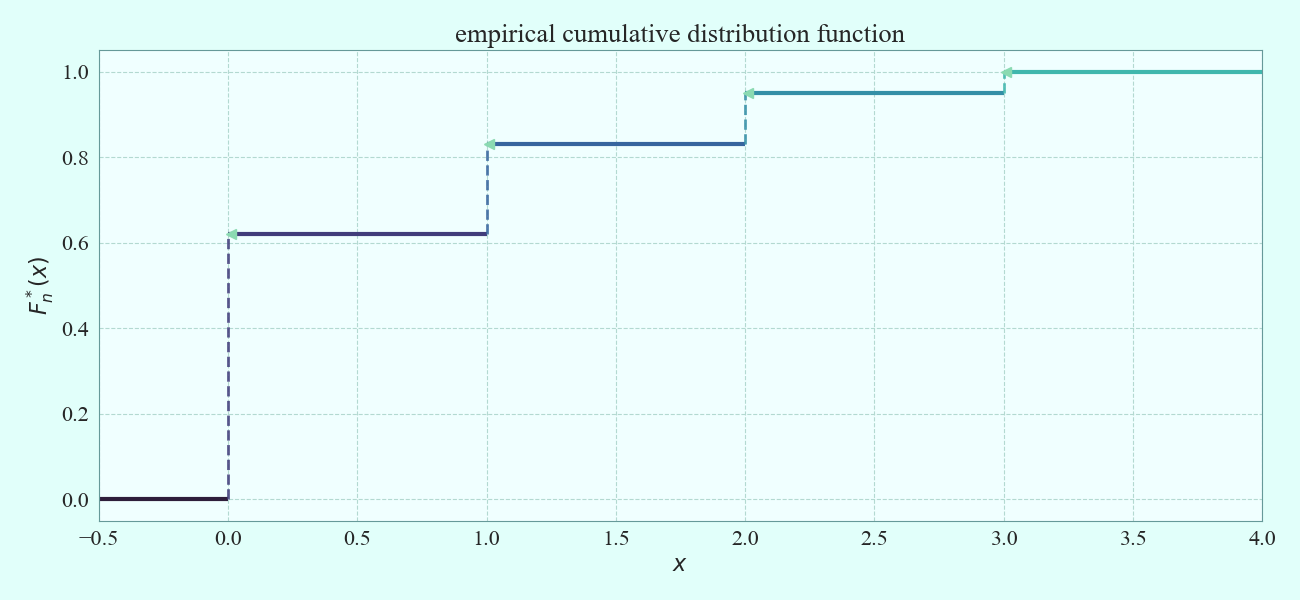
\includegraphics[width={0.8\textwidth}]{../figures/cdf.png}
    \caption{Empirical Cumulative Distribution Function}
    \label{fig:ecdf}
\end{figure}

\begin{figure}[ht]
    \centering
    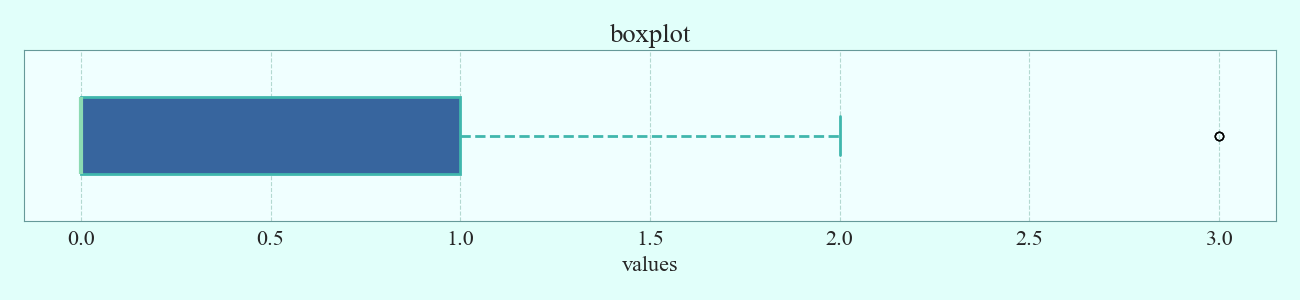
\includegraphics[width={0.8\textwidth}]{../figures/boxplot.png}
    \caption{Box-and-Whisker Plot}
    \label{fig:boxplot}
\end{figure}

\section{Sample Characteristics}

\subsection{Mean and Variance}
By the definition, empirical mean, empirical variance (dispersion), and corrected empirical variance are respectively defined as follows:
\begin{gather*}
\overline{x} = \dfrac{1}{n}\sum\limits_{i=1}^n x_i; \quad \mathbb{D}_{\xi}^{**} = \dfrac{1}{n}\sum\limits_{i = 1}^n (x_i - \overline{x})^2;  \quad \mathbb{D}_{\xi}^{***} = \dfrac{1}{n-1}\sum\limits_{i = 1}^n (x_i - \overline{x})^2.
\end{gather*}
In our case, sample mean equals $\bar{x}=0.6$, suggesting a low-rate counting process.
Having the empirical mean computed, we immediately obtain values for both variances. 
Note that corrected variance may be expressed as the variance with the delta degrees of freedom being equal to one. 
We have: $\mathbb{D}_{\xi}^{**} = 0.7799(9), \  \mathbb{D}_{\xi}^{***} = 0.7878(78)$.

\subsection{Mode, Median, Skewness, and Excess Kurtosis}
Having our sample sorted, we immediately obtain mode and median respectively being equal to zero:
\begin{gather*}
M_e^* = 0, \quad M_0^* = 0.
\end{gather*}
There are various approaches to calculating skewness and kurtosis coefficients.
One of the key aspects of calculation is whether we use corrected variance or not. 
Also, it is important to account for the estimation being biased or not. 
If unbiased, the calculations are corrected for bias and the value computed is 
the adjusted Fisher-Pearson standardized moment coefficient. %ref 
Also, for kurtosis computation, we can specify whether Fisher's definition is used or not, if yes we are substituting three from the final value, and thereby converging to zero. 
The above-defined entities are computed as follows: 

\begin{gather*}
As = \dfrac{\overline{\mu^3}}{s_0^3}, \text{where } \ \overline{\mu^3} = \dfrac{1}{n}\sum\limits_{i = 1}^n(x_i - \overline{x})^3, \text{and } \ s_0^3 = \sqrt{\mathbb{D}_{\xi}^{***}}^3.
\end{gather*}
and 
\begin{gather*}
Ek = \dfrac{\overline{\mu^4}}{s_0^4} - 3, \text{where } \ \overline{\mu^4} = \dfrac{1}{n}\sum\limits_{i = 1}^n(x_i - \overline{x})^4, \text{and } s_0^4 = \sqrt{\mathbb{D}_{\xi}^{***}}^4 = (\mathbb{D}_{\xi}^{***})^2.
\end{gather*}
Note that we use corrected variance for both calculations. After performing tedious arithmetic, we obtain: 
\begin{gather*}
As = 1.286925473140655 \text{ and } Ek = 0.5531041420118363. 
\end{gather*}

\section{Analysis of the Discrete Distributions and Hypothesis Proposal}
We will consider three core discrete distributions: Binomial, Poisson, and Geometric. 
Our approach would be to estimate the parameters based on the empirical quantities 
we have previously computed.

\subsection{Binomial Distribution}
Binomial distribution for a random variable $\xi$ is defined by the number of trials --- $n$,
and the probability of success of a trial --- $p$. Analytically, the expectation and variance are computed as follows:
\begin{gather*}
\mathbb{E}\xi = np, \ \ 
\mathbb{D}\xi = npq, \ \ 
M_e^* \in \{\lfloor np \rfloor \pm 1, \lfloor np \rfloor\}, \ \ 
M_0 = \lfloor (n+1)p \rfloor, \ \ 
As = \dfrac{q - p}{\sqrt{npq}}, \ \ 
Ek = \dfrac{1 - 6pq}{npq}.
\end{gather*}
By using the empirical mean and variance we can approximate the probability of binomial distribution, and thereby compute other characteristic's approximations. 
From the empirical mean we immediately obtain the approximation of the binomial probability $p = 0.2$. 
We have set $n = 3$, as it is the maximum amount of possible successes, as seen from our sample. 

Should we try to approximate probability from variance we would obtain a negative value which strongly contradicts with the probability measure definitions.
Also, it could be easily observed that $\mathbb{E}\xi = np \geq \mathbb{D}\xi = npq$, which is wrong for our sample. 
Finally, with the estimated probability $p = 0.2$ we can compute other estimations. 
For convenience, the data is presented in the table \ref{tab:approx}.

\begin{gather*} 
\mathbb{D}\xi = npq, \ \ 
M_e^* \in \{\lfloor np \rfloor \pm 1, \lfloor np \rfloor\}, \ \ 
M_0 = \lfloor (n+1)p \rfloor, \ \ 
As = \dfrac{q - p}{\sqrt{npq}}, \ \ 
Ek = \dfrac{1 - 6pq}{npq}.
\end{gather*}

\subsection{Poisson Distribution}
Similarly, we can estimate the parameters for the Poisson distribution: 
\begin{gather*}
\mathbb{E}\xi = \mathbb{D}\xi = \lambda, \ \ 
M_e^* = \lfloor \lambda + \dfrac{1}{3} - 0.02\lambda \rfloor, \ \ 
M_0 = \lfloor \lambda \rfloor, \ \ 
As = \dfrac{1}{\sqrt{\lambda}}, \ \ 
Ek = \dfrac{1}{\lambda}.
\end{gather*}


\subsection{Geometric Distribution}
Finally, here are the estimations for the geometric distribution:
\begin{gather*}
\mathbb{E}\xi = \dfrac{q}{p}, \ \ 
\mathbb{D}\xi = \dfrac{q}{p^2}, \ \ 
M_e^* = \left\lceil \dfrac{-1}{\log_2(1-p)}\right\rceil - 1, \ \ 
M_0 = 0, \ \ 
As = \dfrac{2 - p}{\sqrt{1 - p}}, \ \ 
Ek = 6 + \dfrac{p^2}{1 - p}.
\end{gather*}
Note, that we are using the $Geom_0$ variation of the geometric distribution as we have zeros present in our sample. 
Naturally, it means that we are modelling number of failures before the first success in the experiment.

The information about the estimations is gather in the table \ref{tab:approx} for convenience. 
\begin{table}[ht]
\centering
\setlength{\tabcolsep}{10pt}
\renewcommand{\arraystretch}{1.25}
\caption{Estimated characteristics of the fitted distributions}
\label{tab:approx}
\begin{tabular}{llll}
\toprule
characteristic & binomial & poisson & geometric \\
\midrule
parameters 
& $n=3,\ p=0.20$
& $\lambda=0.60$
& $p=0.625$ \\

mean 
& $0.60$
& $0.60$
& $0.60$ \\

variance 
& $0.48$
& $0.60$
& $0.96$ \\

median 
& $\{-1,\ 0,\ 1\}$
& $0$
& $0$ \\

mode 
& $0$
& $0$
& $0$ \\

skewness 
& $0.866$
& $1.291$
& $2.245$ \\

excess kurtosis 
& $0.083$
& $1.667$
& $7.042$ \\
\bottomrule
\end{tabular}
\end{table}

Having the discrete distributions analysed, we shall visualise the 
probability mass functions over the relative frequencies of our sample, as seen on the figure \ref{fig:dists}. 
To achieve that, we have computed the values of probability mass functions for each distribution with the estimated parameters based on the information available from the given sample.

\begin{figure}[ht]
    \centering
    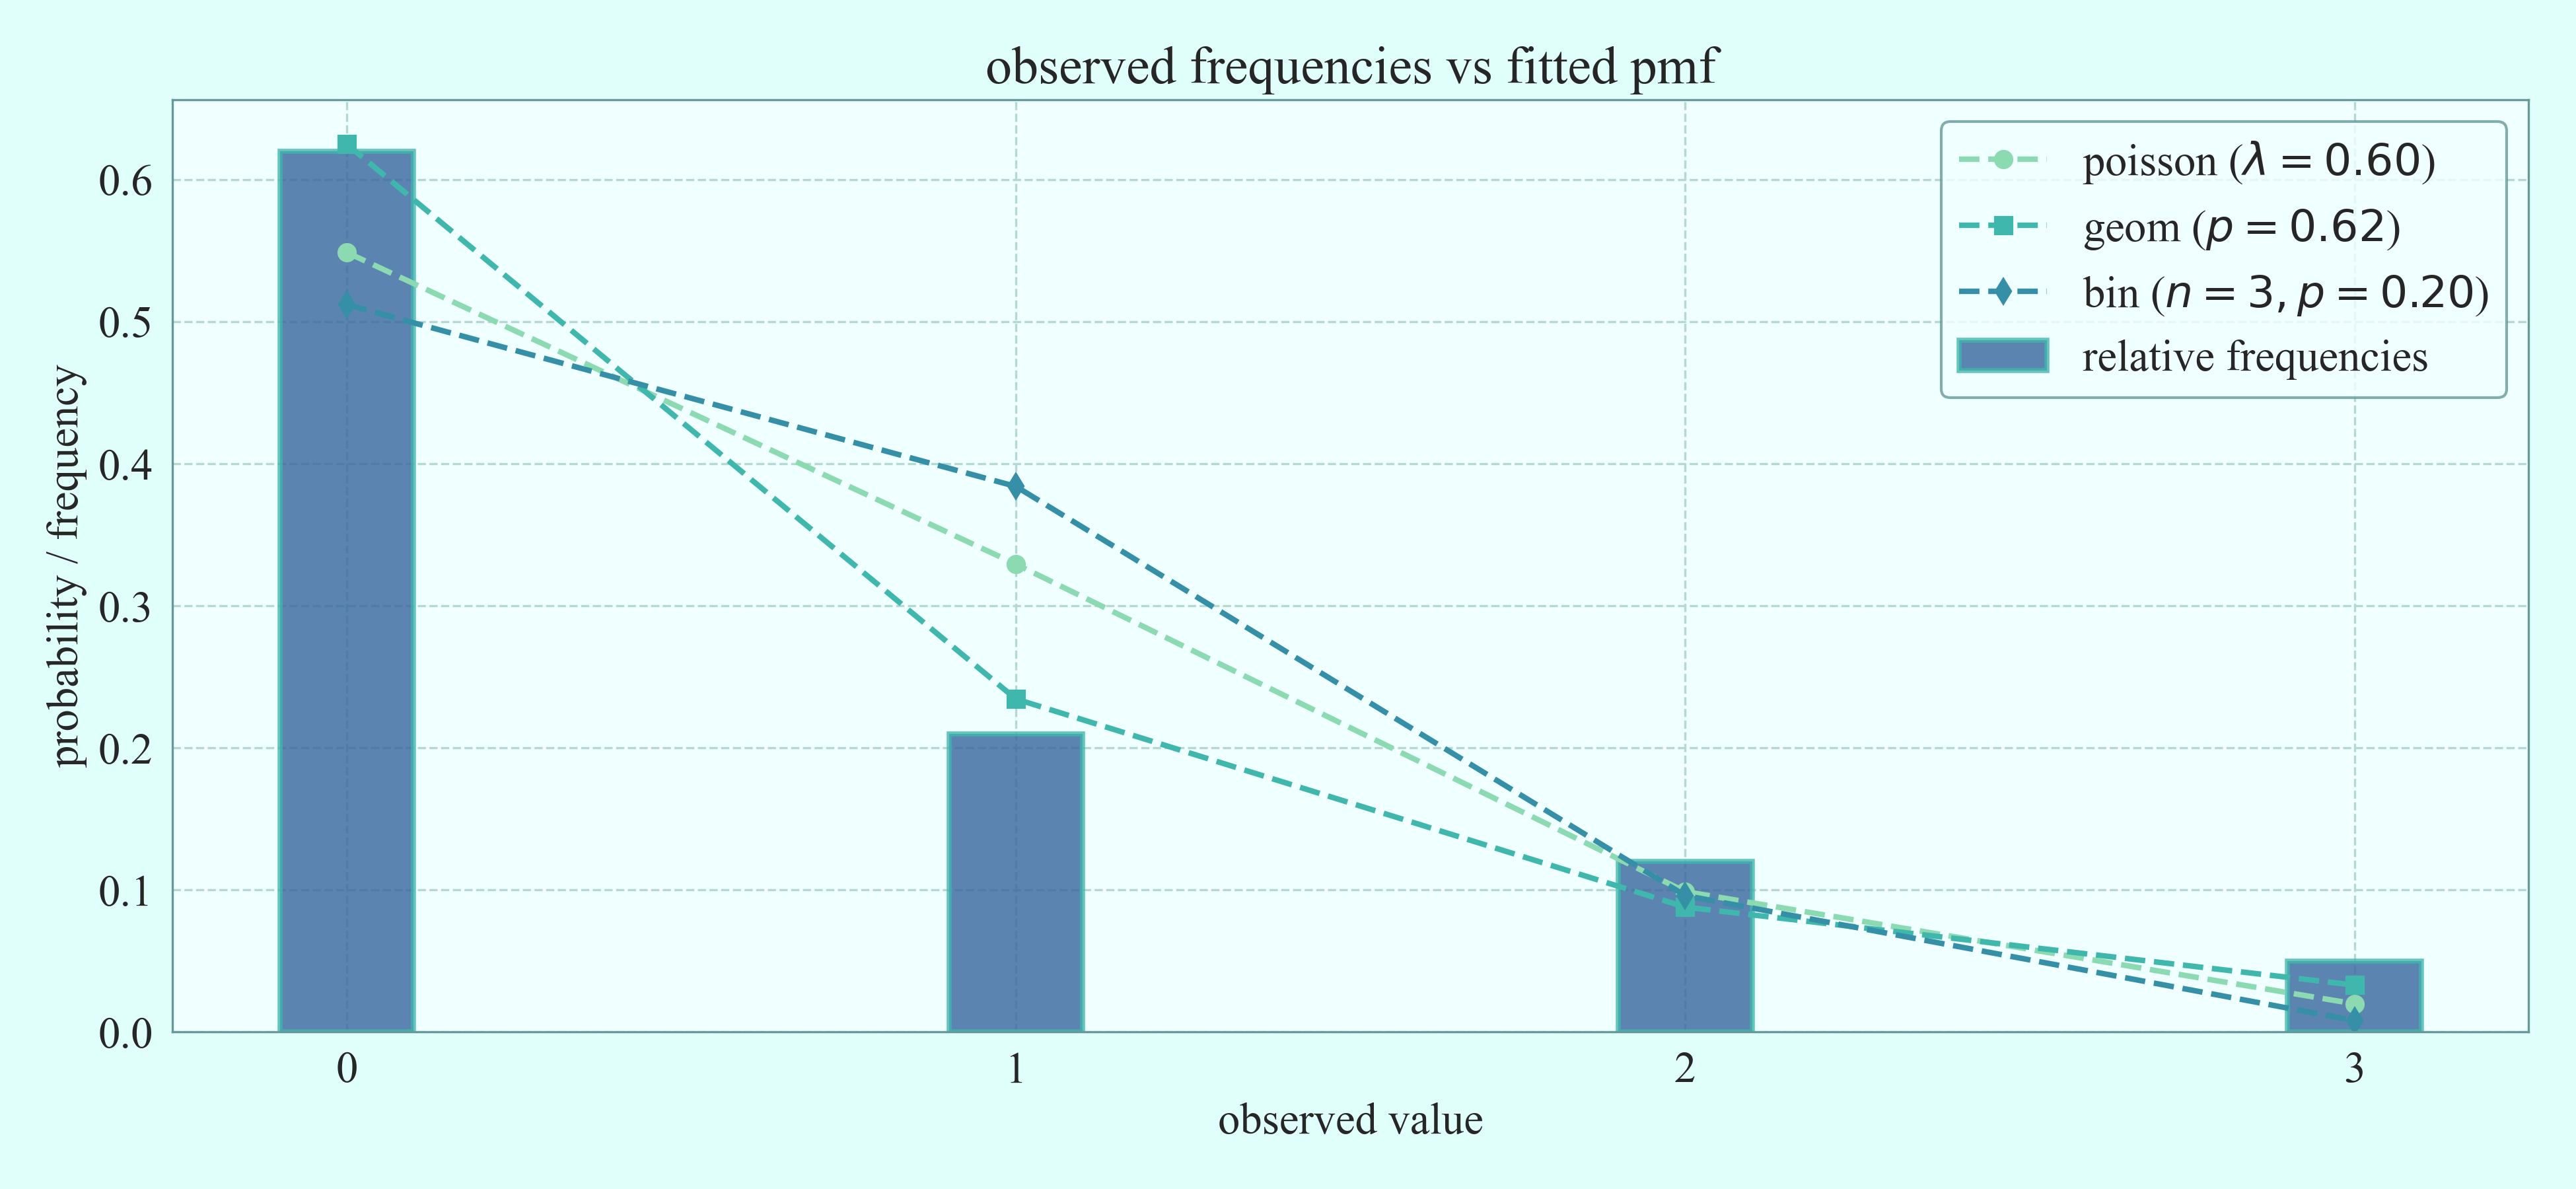
\includegraphics[width={0.8\textwidth}]{../figures/dists.png}
    \caption{Distribution Comparison}
    \label{fig:dists}
\end{figure} 


\subsection{Hypothesis Proposal}

Table~\ref{tab:approx} shows that the Poisson distribution provides the closest match to the sample moments, 
particularly in terms of variance and skewness, 
whereas the binomial model underestimates dispersion and the geometric model overestimates it.

Moreover, interestingly the geometric distribution is the closest in terms of the probability mass function approximation.
Effectively we cannot distinguish which distribution describes the sample in the best way yet. 
Hence, we shall test two hypotheses: 
\begin{gather*}
\xi \thicksim Pois(\lambda) \ \text{ or } \ \xi \thicksim Geom_0(p).
\end{gather*}

\section{Poisson Distribution Analysis}
In this section we will thoroughly investigate the $\lambda$ parameter of the Poisson distribution:
we will construct the estimates of it and perform unbiasedness, consistency, and efficiency checks.
Finally, we will construct asymptotic confidence intervals for the distribution parameter.

\subsection{Method of Moments for the Parameter Estimation}
The most common estimation of the parameter lambda would be the empirical mean, 
which is also the parameter itself:
\begin{gather*}
\lambda^* = \overline{\xi} = \dfrac{\xi_1 + \ldots + \xi_n}{n}.
\end{gather*}
However, obviously, such an estimation would not be suffcient to call it a day. 
Therefore, we shall investigate further. 

\subsection{Maximum Likelihood Method for the Parameter Estimation}
To begin with, we shall construct the maximum likelihood function $L$ by way of multiplication: 
\begin{gather*}
L(\vec{x}, \lambda) = \prod_{i=1}^n \mathbb{P}\{\xi = x_i\} =
\prod_{i=1}^n e^{-\lambda} \cdot \dfrac{\lambda^{x_i}}{x_i!} = 
e^{-n \cdot \lambda} \cdot \dfrac{\lambda^{x_1 + \ldots + x_n}}{x_1! \cdot \ldots \cdot x_n!}.
\end{gather*}
Then, we shall apply natural logarithm from the left over this function: 
\begin{gather*}
\ln L(\vec{x}, \lambda) = 
\ln \left( e^{-n \cdot \lambda} \cdot \dfrac{\lambda^{x_1 + \ldots + x_n}}{x_1! \cdot \ldots \cdot x_n!} \right) =
-n\lambda + (x_1 + \ldots + x_n)\ln \lambda - \ln(x_1! \cdot \ldots \cdot x_n!).
\end{gather*}
Finally, we partially differentiate the expression by lambda, and set the expression to zero: 
\begin{gather*}
\dfrac{\partial \ln L(\vec{x}, \lambda)}{\partial \lambda} =
 -n + \dfrac{x_1 + \ldots + x_n}{\lambda} = 0 \quad \Longrightarrow \quad \lambda^* =
\dfrac{x_1 + \ldots + x_n}{n} = \overline{x}.
\end{gather*}
Both methods yielded the same estimation --- empirical mean of the sample. 
This approximation is rather trivial. However, as the empirical mean is the parameter itself, 
it makes perfect sense to use is as the estimation. We have formally proved that. 

\subsection{Evaluation of Unbiasedness, Consistency, and Efficiency}
Having the parameter estimated, we need to formally check its characteristics that would make
a solid estimation, as otherwise it would not be reliable. 

\subsubsection{Unbiasedness}
An estimation of a parameter is unbiased if the following condition is true: 
\begin{gather*}
\mathbb{E}\lambda^* = \lambda.
\end{gather*}
Hence, for our case:
\begin{gather*}
\mathbb{E}\lambda^* =
\mathbb{E} \left(\dfrac{\xi_1 + \ldots + \xi_n}{n}\right) = 
\dfrac{1}{n}\cdot \mathbb{E}\left(\xi_1 + \ldots + \xi_n \right) = 
\dfrac{1}{n} \left( \mathbb{E}\xi_1 + \ldots + \mathbb{E}\xi_n \right) = 
\dfrac{1}{n} \cdot n\lambda = \lambda.
\end{gather*}
We can confidently state that the obtained estimation is unbiased. 

\subsubsection{Consistency}
An estimation of a parameter is consistent if the following condition is true: 
\begin{gather*}
\lambda^*_n \xrightarrow[n \to + \infty]{\mathbb{P}, \ \text{ a. s.}} \lambda.
\end{gather*}
To prove that we shall apply the strong law of large numbers that says that the empirical mean
converges to the analytical expectation: 
\begin{gather*}
\lim\limits_{n \to \infty}\lambda^*_n = \lim\limits_{n \to \infty}  \left(\dfrac{\xi_1 + \ldots + \xi_n}{n}\right) = \mathbb{E}\xi = \lambda.
\end{gather*}
This expression proves the consistency of the parameter estimation.

\subsubsection{Efficiency}

Since the obtained estimator $\lambda^*$ is unbiased, it follows from the criterion for efficiency that it suffices to verify that, in the following identity, the constant $C$ does not depend on $\mathbf{x}$ or on $\lambda^*(\mathbf{x})$:
\begin{gather*}
\frac{\partial}{\partial \lambda} \ln L(\mathbf{x}, \lambda) = C \cdot \bigl[\lambda^*(\mathbf{x}) - \lambda\bigr].
\end{gather*}
In our case, we have:
\begin{gather*}
-n + \frac{x_1 + \cdots + x_n}{\lambda}
= C \cdot \left[\frac{x_1 + \cdots + x_n}{n} - \lambda \right]
\quad
\Longrightarrow
\quad
C =
\frac{\dfrac{x_1 + \cdots + x_n - n\lambda}{\lambda}}
{\dfrac{x_1 + \cdots + x_n - n\lambda}{n}}
= \frac{n}{\lambda}.
\end{gather*}

Thus, the estimator $\lambda^* = \bar{x}$ is unbiased, consistent, and efficient, and therefore achieves the Cramér–Rao lower bound for the Poisson model.

\subsection{Asymptotic Confidence Intervals Construction}
We now construct an asymptotic confidence interval for the parameter $\lambda$ with confidence level $\gamma = 0.95$.
By the Central Limit Theorem, the estimator $\lambda^*$ is approximately normally distributed:
\begin{gather*}
\lambda^* = \bar{\xi} = \frac{\xi_1 + \cdots + \xi_n}{n} \approx N\!\left(\lambda, \frac{\lambda}{n}\right).
\end{gather*}
Since, under the Poisson modelling assumption $\mathbb{E}[\lambda^*] = \lambda, \mathbb{D}[\lambda^*] = \dfrac{\lambda}{n},$
we obtain the following approximation:
\begin{gather*}
\frac{\lambda^* - \lambda}{\sqrt{\lambda / n}}
= \sqrt{n}\,\frac{\lambda^* - \lambda}{\sqrt{\lambda}}
\approx N(0,1).
\end{gather*}
By definition of an approximate confidence interval with confidence level $\gamma$, we have:
\begin{gather*}
\mathbb{P}\left\{
- t_{\gamma} 
< \sqrt{n}\,\frac{\lambda^* - \lambda}{\sqrt{\lambda}}
< t_{\gamma}
\right\}
\approx \gamma = 0.95.
\end{gather*}
Here $t_{\gamma}$ is the $(1+\gamma)/2$ quantile of the standard normal distribution:
\begin{gather*}
\Phi(t_{\gamma}) = \frac{1+\gamma}{2},
\qquad t_{\gamma} = 1.96.
\end{gather*}
Now, we solve the obtained inequality for $\lambda$:
\begin{gather*}
n \cdot \dfrac{(\lambda^* - \lambda)^2}{\lambda} < t_{\gamma}^2 \ \Longrightarrow \ 
(\lambda^* - \lambda)^2 < \dfrac{\lambda \cdot t_{\gamma}^2}{n} \ \Longrightarrow \ 
\lambda^2 - 2\lambda^*\lambda + (\lambda^*)^2 - \dfrac{\lambda \cdot t_{\gamma}^2}{n} < 0
\end{gather*}
and find the roots of the quadratic equation: 
\begin{gather*}
D = \left(2\lambda^* + \dfrac{t_{\gamma}^2}{n}\right)^2 - 4(\lambda^*)^2 = 4(\lambda^*)^2 + 4\left(\dfrac{t_{\gamma}^2 \cdot \lambda^*}{n}\right) + \dfrac{t_{\gamma}^4}{n^2} - 4(\lambda^*)^2 = t_{\gamma}^2 \left(\dfrac{4\lambda^*}{n} + \dfrac{t_{\gamma}^2}{n^2}\right).
\\
\lambda_{1, 2}^* = \dfrac{2\lambda^* + \dfrac{t_{\gamma}^2}{n} \pm t_{\gamma}\sqrt{\dfrac{4\lambda^*}{n} + \dfrac{t_{\gamma}^2}{n^2}}}{2} = \lambda^* + \dfrac{t_{\gamma}^2}{2n} \pm t_{\gamma} \sqrt{\dfrac{\lambda^*}{n} + \dfrac{t_{\gamma}^2}{4n^2}}.
\end{gather*}
Finally, we obtain an approximate confidence interval for the parameter $\lambda$: 
\begin{gather*}
\left(
    \lambda^* + \dfrac{t_{\gamma}^2}{2n} - t_{\gamma} \sqrt{\dfrac{\lambda^*}{n} + \dfrac{t_{\gamma}^2}{4n^2}}, \quad
    \lambda^* + \dfrac{t_{\gamma}^2}{2n} + t_{\gamma} \sqrt{\dfrac{\lambda^*}{n} + \dfrac{t_{\gamma}^2}{4n^2}}
\right) 
\end{gather*}
Computationally, we obtain an interval of the form $(0.4661768029714202, 0.7722391970285798) \ni \lambda$.

\section{Geometric Distribution Analysis} 
Similarly to the previous section, here we will estimate the parameter of the geometric distribution $p$,
and perform the same analysis we did.
We will investigate the geometric distribution in the following form: 
\begin{gather*}
\mathbb{P}\{\xi = k \} = \dfrac{a^k}{(a+1)^{k+1}} = 
\dfrac{1}{a+1} \cdot \left(\dfrac{a}{a+1}\right)^k = pq^k.
\end{gather*}

\subsection{Method of Moments for the Parameter Estimation}
Method of moments trivially yields the following estimation:
\begin{gather*}
\mathbb{E}\xi = \dfrac{q}{p} = \dfrac{\dfrac{a}{a+1}}{\dfrac{1}{a+1}} =
a, \quad \overline{\xi} = a^*.
\end{gather*}

\subsection{Maximum Likelihood Method for the Parameter Estimation}
Analogously, we construct the maximum likelihood function: 
\begin{gather*}
L(x_1, \ldots, x_n, a) = \prod\limits_{i = 1}^{n}\mathbb{P}\{ \xi = x_i \} = 
\prod\limits_{i = 1}^{n} \dfrac{a^{x_i}}{(a+1)^{x_i +1}} = 
\dfrac{a^{\sum x_i}}{(a+1)^{\sum x_i + n}}.
\end{gather*}
Then, we apply natural logarithm to the constructed function:
\begin{gather*}
\ln L(x_1, \ldots, x_n, a) =
 \sum\limits_{i = 1}^n x_i \ln a - \left(\sum\limits_{i = 1}^n x_i + n \right)\ln(a + 1).
\end{gather*}
Consequently, we partially differentiate by the parameter $a$:  
\begin{gather*}
\dfrac{\partial}{\partial a}\ln L(x_1, \ldots, x_n, a)
=
\dfrac{\sum_{i=1}^n x_i}{a}
-
\dfrac{\sum_{i=1}^n x_i + n}{a+1}
= 0
\quad \Longrightarrow \quad
a^* = \dfrac{\sum_{i=1}^n x_i}{n} = \overline{x}.
\end{gather*}
Similarly, both methods yielded the same approximation --- empirical mean. 

\subsection{Evaluation of Unbiasedness, Consistency, and Efficiency}

\subsubsection{Unbiasedness}
We first verify that the estimator $a^* = \overline{\xi}$ is unbiased. 
By definition, an estimator is unbiased if its expectation equals the true parameter value.
\begin{gather*}
\mathbb{E}\overline{\xi} = \frac{1}{n} \sum_{i=1}^n \mathbb{E}\xi_i = a.
\end{gather*}
Thus, the sample mean coincides with the expectation of the distribution, and the estimator $a^*$ is unbiased.

\subsubsection{Consistency}
Next, we establish consistency of the estimator. An estimator is consistent if it converges to the true parameter value as the sample size increases.
\begin{gather*}
a^*_n = \dfrac{\sum\limits_{i = 1}^n x_i}{n} \quad 
\xrightarrow[n \to + \infty]{\mathbb{P}, \ \text{a.s.}} \quad \mathbb{E}\xi_k = a.
\end{gather*}
By the Law of Large Numbers, the sample mean converges (both in probability and almost surely) to the expected value of the distribution. Therefore, $a^*$ is a consistent estimator.

\subsubsection{Efficiency}
Finally, we verify efficiency using the standard criterion: 
for an efficient estimator, the derivative of the likelihood can be expressed as 
a constant multiple of $(a^* - a)$.
\begin{gather*}
\dfrac{\partial}{\partial a} L(x_1, \ldots, x_n, a) \stackrel{?}{=} C(a^* - a).
\end{gather*}
We compute the derivative explicitly:
\begin{gather*}
\dfrac{\partial}{\partial a} L(x_1, \ldots, x_n, a) = 
\dfrac{\sum\limits_{i = 1}^n x_i}{a} - \dfrac{\sum\limits_{i = 1}^n x_i + n}{a + 1} 
= \dfrac{a\sum\limits_{i = 1}^n x_i + \sum\limits_{i = 1}^n x_i - a \sum\limits_{i = 1}^n x_i - an}{a(a+1)} 
= \dfrac{ \sum\limits_{i = 1}^n x_i - an}{a(a+1)}.
\end{gather*}
On the other hand, we express $(a^* - a)$ and match both expressions, we obtain:
\begin{gather*}
C(a^* - a) = C\left(\dfrac{\sum\limits_{i = 1}^n x_i - an}{n} \right). 
\Longrightarrow
\dfrac{ \sum\limits_{i = 1}^n x_i - an}{a(a+1)} = 
C \cdot \dfrac{\sum\limits_{i = 1}^n x_i - an}{n}
\quad \Longrightarrow \quad 
C = \dfrac{n}{a(a + 1)}.
\end{gather*}
Since the derivative of the likelihood can be written in the required form with a constant $C$ independent of the data, the estimator $a^*$ is efficient and attains the Cramér--Rao lower bound.

\subsection{Asymptotic Confidence Intervals Construction}
To construct a confidence interval for the parameter $a$, we apply the Central Limit Theorem (CLT). 
For sufficiently large $n$, the estimator $a^*$ is approximately normally distributed:
\begin{gather*}
\dfrac{a^* - \mathbb{E}a^*}{\sqrt{\mathbb{D}a^*}} \approx N(0, 1).
\end{gather*}
We already know that:
\begin{gather*}
\mathbb{E}a^* = a, \quad 
\mathbb{D}a^* = \dfrac{1}{n}\mathbb{D}\xi.
\end{gather*}
For the geometric distribution under consideration, we have:
\begin{gather*}
\mathbb{D}\xi = \dfrac{q}{p^2}.
\end{gather*}
Using the parametrisation $p = \dfrac{1}{a + 1}$ and $q = 1 - p = \dfrac{a}{a+1}$, we obtain:
\begin{gather*}
\mathbb{D}a^* = \dfrac{1}{n} \cdot \dfrac{q}{p^2}
= \dfrac{1}{n} \cdot \dfrac{\frac{a}{a+1}}{\frac{1}{(a+1)^2}}
= \dfrac{a^2 + a}{n}.
\end{gather*}
Substituting into the CLT expression, we get:
\begin{gather*}
\dfrac{a^* - a}{\sqrt{(a^2 + a)/n}} 
= \dfrac{\sqrt{n}(a^* - a)}{\sqrt{a^2 + a}} 
\approx N(0, 1).
\end{gather*}
We now write the probability statement corresponding to a confidence level $\gamma = 0.95$:
\begin{gather*}
\mathbb{P}\left\{ 
- t_{\gamma} < 
\dfrac{\sqrt{n}(a^* - a)}{\sqrt{a^2 + a}} 
< t_{\gamma}
\right\} \approx \gamma.
\end{gather*}
To obtain an explicit confidence interval for $a$, we square both sides of the inequality and rearrange:
\begin{gather*}
\dfrac{n(a^* - a)^2}{a^2 + a} < t_{\gamma}^2.
\end{gather*}
This leads to a quadratic inequality in $a$:
\begin{gather*}
a^2\left(1 - \dfrac{t_{\gamma}^2}{n}\right) 
- a\left(2a^* + \dfrac{t_{\gamma}^2}{n}\right) 
+ (a^*)^2 < 0.
\end{gather*}
To solve it, we compute the discriminant:
\begin{gather*}
D = t_{\gamma}^2\left(
\dfrac{t_{\gamma}^2}{n^2} + \dfrac{4a^*(a^* + 1)}{n}
\right).
\end{gather*}
Finally, the roots of the quadratic equation are:
\begin{gather*}
a_{1,2} = 
\dfrac{
2a^* + \dfrac{t_{\gamma}^2}{n} 
\pm 
t_{\gamma}\sqrt{
\dfrac{t_{\gamma}^2}{n^2} + \dfrac{4a^*(a^* + 1)}{n}
}
}{
2\left(1 - \dfrac{t_{\gamma}^2}{n}\right)
}.
\end{gather*}
Computationally, 
the approximate interval for $a$ is given by $(0.49983101048836076, 0.7880606349633106) \ni a$.

\section{Chi-Squared Tests}
We will test both of our hypotheses on two significance levels: $\alpha = 0.05$ and $\alpha = 0.01$
For testing we will calculate the Chi-Square value as follows:
\begin{gather}
\label{eq:chi2}
\scalebox{1.5}{$\chi$}^2(n) = \sum\limits_{i = 1}^m \dfrac{(n_i - np_i)^2}{np_i}.
\end{gather}
Also, for the case of a composite hypothesis, the test statistic follows the distribution: 
$\scalebox{1.5}{$\chi$}^2_{m - s - 1, \ \alpha}$ with $m - s - 1$ degrees of freedom and significance level $\alpha$.

\subsection{Poisson Hypothesis Evaluation}
The first hypothesis to test is:
\begin{gather*}
H_0: \xi \sim Pois
\end{gather*}
We have combined bins for values 2 and 3 into one, as separately they have 
to small expectation value. The table \ref{tab:chi_poisson} 
shows the intermediate and calculated values of the chi-square statistic for the Poisson distribution.
\begin{table}[ht!]
\centering
\setlength{\tabcolsep}{10pt}
\renewcommand{\arraystretch}{1.25}
\caption{Chi-square goodness-of-fit test for the Poisson distribution}
\label{tab:chi_poisson}
\begin{tabular}{llll}
\toprule
$\Delta_i$ & $n_i$ & $p_i$ & $\chi^2_i$ \\
\midrule
$0$ 
& $62$ 
& $0.54881$ 
& $0.9234$ \\

$1$ 
& $21$ 
& $0.32929$ 
& $4.3208$ \\

$\geq 2$ 
& $17$ 
& $1 - 0.54881 - 0.32929 = 0.12190$ 
& $1.8973$ \\

\midrule
\multicolumn{3}{r}{total} & $7.1415$ \\
\bottomrule
\end{tabular}
\end{table}
In case of the significance level $\alpha = 0.05$ and 1 degree of freedom we have:
\begin{gather*}
\scalebox{1.5}{$\chi$}^2_{m - s - 1, \ \alpha} = \scalebox{1.5}{$\chi$}^2_{3 - 1 - 1, \ 0.95} = \scalebox{1.5}{$\chi$}^2_{1, \ 0.95} =  3.8415 < 7.1415 = \scalebox{1.5}{$\chi$}^2(n).
\end{gather*}
Furthermore, for the significance level $\alpha = 0.01$: 
\begin{gather*}
\scalebox{1.5}{$\chi$}^2_{m - s - 1, \ \alpha} = \scalebox{1.5}{$\chi$}^2_{3 - 1 - 1, \ 0.99} = \scalebox{1.5}{$\chi$}^2_{1, \ 0.99} =  6.635 < 7.1415 = \scalebox{1.5}{$\chi$}^2(n).
\end{gather*}
Hence, both on the significance level $\alpha = 0.05$ and  $\alpha = 0.01$ we reject the Poisson hypothesis.


\subsection{Geometric Hypothesis Evaluation}
The latter hypothesis we test is: 
The table \ref{tab:chi_geometric} 
shows the intermediate and calculated values of the chi-square statistic for the Geometric distribution.
Here, we have more bins, resulting in two degrees of freedom. 
\begin{gather*}
H_0: \xi \sim Geom_0
\end{gather*}
\begin{table}[ht]
\centering
\setlength{\tabcolsep}{10pt}
\renewcommand{\arraystretch}{1.25}
\caption{Chi-square goodness-of-fit test for the Geometric distribution}
\label{tab:chi_geometric}
\begin{tabular}{llll}
\toprule
$\Delta_i$ & $n_i$ & $p_i$ & $\chi^2_i$ \\
\midrule
$0$ 
& $62$ 
& $0.625$ 
& $0.0040$ \\

$1$ 
& $21$ 
& $0.23438$ 
& $0.2536$ \\

$2$ 
& $12$ 
& $0.08789$ 
& $1.1742$ \\

$\geq 3$ 
& $5$ 
& $1 - 0.625 - 0.23438 - 0.08789 = 0.05273$ 
& $0.0142$ \\

\midrule
\multicolumn{3}{r}{total} & $1.4447$ \\
\bottomrule
\end{tabular}
\end{table}
As we now operate with 2 degrees of freedom the chi-square statistics would be of the form
\begin{gather*}
\scalebox{1.5}{$\chi$}^2_{m - s - 1, \ \alpha} = \scalebox{1.5}{$\chi$}^2_{4 - 1 - 1, \ 0.95} = \scalebox{1.5}{$\chi$}^2_{2, \ 0.95} =  5.991 > 1.445 = \scalebox{1.5}{$\chi$}^2(n),
\end{gather*}
and
\begin{gather*}
\scalebox{1.5}{$\chi$}^2_{m - s - 1, \ \alpha} = \scalebox{1.5}{$\chi$}^2_{4 - 1 - 1, \ 0.99} = \scalebox{1.5}{$\chi$}^2_{2, \ 0.99} =  9.210 > 1.445 = \scalebox{1.5}{$\chi$}^2(n).
\end{gather*}
For both significance levels we can clearly state that the proposed hypothesis does not contradict with the observations, and thereby could be accepted.

\section{Discussions \& Conclusions}

\subsection{Limitations of the Models}
The Poisson model assumes equidispersion, i.e.\ $\mathbb{E}\xi = \mathbb{D}\xi$. 
In our data, the variance is noticeably larger than the mean, indicating overdispersion. 
This directly contradicts the assumptions of the Poisson model and explains its poor fit.
The geometric distribution assumes a memoryless process, which does not have a clear interpretation in this setting. 
However, it provides a more flexible shape, in particular a heavier tail, which allows it to better match the observed data.

\subsection{Interpretation and Comparison}

The empirical distribution is strongly concentrated at zero but still exhibits a non-negligible tail. 
The Poisson model decays too quickly and underestimates larger values, which leads to a significant discrepancy in the chi-square test.
In contrast, the geometric distribution assigns more mass to higher values and captures the overall shape of the data more accurately. 
As a result, it is not rejected by the chi-square test and provides a better empirical fit.
At the same time, the observed overdispersion suggests that the data may arise from a more complex mechanism, 
for example a mixture of processes or heterogeneous event rates, which cannot be captured by the Poisson model.

\subsection{Conclusions}

The Poisson model is rejected at standard significance levels, while the geometric model is not. 
Therefore, among the considered options, the geometric distribution provides a more adequate description of the data.
However, neither model should be interpreted as the true underlying mechanism. 
The presence of overdispersion indicates that more flexible models, such as the negative binomial distribution, 
are likely to provide a better fit and represent a natural direction for further study.

\section*{Acknowledgements}

The author is grateful to Prof. Andrii Ilienko for guidance and valuable discussions related to mathematical statistics.
Also, I would like to mention the extensive effects of caffeine and sugar, alongside feeling for recognition 
that were keeping me somewhat disciplined while working on this project.

\bibliographystyle{siam}
\bibliography{references.bib}

\end{document}